\documentclass[aps, pre, onecolumn, nofootinbib, notitlepage, groupedaddress, amsfonts, amssymb, amsmath, longbibliography, superscriptaddress]{revtex4-1}
\usepackage{tabularx}
\usepackage{graphicx}
\usepackage{hyperref}
\usepackage{xcolor}
\hypersetup{
    colorlinks,
    linkcolor={red!50!black},
    citecolor={blue!50!black},
    urlcolor={blue!80!black}
}
\usepackage{bm}
\usepackage{natbib}
\usepackage{longtable}
\LTcapwidth=0.87\textwidth

\newcommand{\Div}[1]{\ensuremath{\nabla\cdot\left( #1\right)}}
\newcommand{\DivU}{\ensuremath{\nabla\cdot\bm{u}}}
\newcommand{\angles}[1]{\ensuremath{\left\langle #1 \right\rangle}}
\newcommand{\KS}[1]{\ensuremath{D_{\text{KS}}(#1)}}
\newcommand{\KSstat}[1]{\ensuremath{\overline{D_\text{KS}(#1)}}}
\newcommand{\grad}{\ensuremath{\nabla}}
\newcommand{\RB}{Rayleigh-B\'{e}nard }
\newcommand{\Reff}{\ensuremath{\text{Re}_{\text{ff}}}}
\newcommand{\Peff}{\ensuremath{\text{Pe}_{\text{ff}}}}


\newcommand\mnras{{MNRAS}}%
\newcommand\apjl{{The Astrophysical Journal Letters}}%

\begin{document}
\author{Evan H. Anders}
\affiliation{Dept. Astrophysical \& Planetary Sciences, University of Colorado -- Boulder, Boulder, CO 80309, USA}
\affiliation{Laboratory for Atmospheric and Space Physics, Boulder, CO 80303, USA}
\author{Geoffrey M. Vasil}
\affiliation{University of Sydney School of Mathematics and Statistics, Sydney, NSW 2006, Australia}
\author{Benjamin P. Brown}
\affiliation{Dept. Astrophysical \& Planetary Sciences, University of Colorado -- Boulder, Boulder, CO 80309, USA}
\affiliation{Laboratory for Atmospheric and Space Physics, Boulder, CO 80303, USA}
\author{Lydia Korre}
\affiliation{Laboratory for Atmospheric and Space Physics, Boulder, CO 80303, USA}
\author{Jeffrey S. Oishi}
\affiliation{Department of Physics and Astronomy, Bates College, Lewiston, ME 04240, USA}

\title{Thermal relaxation is important in convective simulations: \\
on the time evolution of flows and how to avoid unnecessary thermal rundown}

\begin{abstract}
Astrophysical simulations of convection frequently impose different thermal boundary conditions at the top and the bottom of the domain in an effort to more accurately reflect the natural system being modeled.
In this work, we study \RB convection (RBC) to understand how mixed (``FT'') thermal boundary conditions, which are often used in astrophysics, change the nature of the convective solution compared to the traditional choice of fixing the temperature at the top and bottom of the domain (``TT'').
We find that FT boundaries impose a long thermal rundown on convective systems which is not experienced by experiments with TT boundaries.
In the evolved state, the mean behavior of an FT simulation corresponds to an equivalent simulation with TT boundaries, and the fast evolution of TT simulations can be taken advantage of to rapidly relax FT simulations.
We show that these findings carry over to more complicated problems through a brief examination of rotating convection.
We furthermore find that FT boundaries introduce minor asymmetries into the flow fields, with the fixed flux boundary producing more extreme events than the fixed temperature boundary, but that these asymmetries do not appreciably affect the bulk flows.
We conclude that thermal relaxation occurs in two stages: (1) changes to the experimental energy reservoir and (2) changes to the stratification of the experiment.
Through the proper choice of boundary conditions or initial conditions, the first of these stages can be bypassed, and the second stage seems to be irrelevant for RBC.
\end{abstract}
\maketitle

%%%%%%%%%%%%
%%%%%%%%%%%
% INTRO
%%%%%%%%%%%
%%%%%%%%%%%%

\section{Introduction}
\label{sec:introduction}
Convection is a crucial heat transport mechanism in the atmospheres and interiors of stars and planets.
Numerical simulations are a commonly-used tool in studies into the nature of convection.
These studies range from examinations of convection in the simplified Boussinesq approximation \cite{spiegel&veronis1960, ahlers&all2009, plumley&julien2019} to highly complex ``dynamo simulations'' which include magnetism and atmospheric density stratification \cite{charbonneau2014, toomre2019}.
In these simulations, convection is fundamentally driven by some combination of imposed boundary conditions and internal heating profiles \cite{goluskin2015}.
One common choice of thermal boundary conditions in astrophysical convection \cite{glatzmaier&gilman1982, hurlburt&all1986, cattaneo&all1990, featherstone&hindman2016a, korre&all2019, wood&brummell2018, kapyla&all2019} is to fix the flux at the bottom boundary and to fix the value of a thermodynamic quantity (e.g., temperature or entropy) at the top boundary.
However, in Boussinesq studies of \RB convection, the most frequently-utilized choice of boundary conditions is to fix the temperature at both boundaries.
We are unaware of any study which has examined the consequences of imposing the ``mixed'' boundaries that are frequently favored in astrophysical convection studies.

In this work, we examine how the choice of using ``mixed'' boundaries affects the evolved nonlinear convective state in the simplest possible model: \RB convection (RBC) under the Boussinesq approximation.
In RBC, temperature is the only thermodynamic quantity and throughout this work we will refer to the choice of fixing the flux at the bottom and temperature at the top as ``FT'' boundary conditions.
We will refer to the common choice of fixing temperature at both boundaries as ``TT'' boundaries, and fixing the flux at both boundaries as ``FF'' boundaries\footnote{Note, in ref.~\cite{goluskin2015}, our TT, FF, and FT are repsectively called RB1, RB2, and RB3.}.
It is generally assumed that FT and FF boundaries should fundamentally behave similarly \cite{goluskin2015}, and the behavior of FF boundaries is well-known \cite{otero&all2002, johnston&doering2009}.
The scaling of the convective heat transport, quantified by the Nusselt number, as a function of increased convective driving, quantified by the Rayleigh number, has been shown to be equivalent for FF and TT boundaries \cite{johnston&doering2009}, and it is natural to assume that FT should fall on the same scaling laws.
However, FT boundaries introduce complexities into the convective solution which neither FF nor TT boundaries are exposed to.
First, the evolved mean temperature of a simulation with FT boundaries differs from the initial mean temperature, and therefore the thermal reservoir of the convective system must evolve over time \cite{anders&all2018}.
Second, FT boundary conditions are fundamentally asymmetric, and it is unclear if these asymmetries affect the evolved convective solution.

In this paper, we investigate the time evolution and nature of asymmetries in \RB covection when FT boundary conditions are imposed, and we compare evolved FT solutions to the most commonly studied TT solutions.
We find that the thermal evolution and relaxation of FT systems is very long compared to TT systems, where it is nearly instantaneous.
However, this long thermal evolution can be bypassed by using the results of TT simulations as initial conditions for FT simulations.
We also find that during their thermal relaxation, FT simulations simulations perform a sweep through parameter space, effectively sampling dynamics at various values of the Rayleigh number over their evolution.
Finally, our results suggest that the choice of FT boundaries imposes some asymmetries on the convective flows, but that these asymmetries do not importantly change the mean convective state when compared to TT siulations.

We present these findings as follows.
In section \ref{sec:simulations}, we describe our simulation setup and numerical methods.
In section \ref{sec:2d_results}, we first describe our findings with respect to the time evolution of FT systems, and then describe the asymmetries in these systems.
In section \ref{sec:rotating_results}, we show that these findings carry over to a more complex system: rotating \RB convection.
Finally, in section \ref{sec:discussion}, we summarize our findings and briefly describe the implications of this work for the field of astrophysical convection.

%%%%%%%%%%%%
%%%%%%%%%%%
% EXPERIMENT
%%%%%%%%%%%
%%%%%%%%%%%%

\section{Simulation Details}
\label{sec:simulations}
We study incompressible \RB convection under a freefall nondimensionalization as we have done previously \cite{anders&all2018}; for details of the nondimensionalization, we refer readers to that previous work.
In section \ref{sec:rotating_results} we study convection which includes the effects of vertical global rotation \cite{julien&all1996}, so here we include the Coriolis term in the momentum equation for generality.
The Boussinesq equations of motion are
\begin{align}
\Div{\bm{u}} &= 0
	\label{eqn:incompressible}
\\
\frac{\partial \bm{u}}{\partial t} + \left(\bm{\omega} + \frac{1}{\text{Ek }\Reff}\hat{z}\right)\times\bm{u} 
&= - \grad \varpi + T_1\hat{z} - \frac{1}{\Reff}\grad\times\bm{\omega},
	\label{eqn:bouss_momentum}
\\
\frac{\partial T_1}{\partial t}  + \bm{u}\cdot\grad T_1 + w \frac{\partial T_0}{\partial z} 
&= \frac{1}{\Peff}\grad^2 T_1,
	\label{eqn:bouss_energy}
\end{align}
where $\bm{u} = (u, v, w)$ is the velocity, $T = T_0(z) + T_1(x, y, z, t)$ is the temperature (where $T_0$ is the initial profile and $T_1$ are the fluctuations around that profile), $\varpi$ is the reduced kinematic pressure \cite{anders&all2018} which enforces the incompressibility constraint, and $\bm{\omega} = \grad \times \bm{u}$ is the vorticity.
The dimensionless control parameters are the Rayleigh (Ra), Prandtl (Pr), and Ekman (Ek) numbers, defined respectively as
\begin{equation}
\text{Ra} = \frac{g \alpha L_z^3 \Delta}{\nu\kappa} = \frac{(L_z\,v_{\text{ff}})^2}{\nu\kappa}, \qquad \text{Pr} = \frac{\nu}{\kappa}, \qquad \text{Ek} = \frac{\nu}{2\Omega L_z^2},
\end{equation}
where $g$ is the gravity, $\alpha$ is the coefficient of thermal expansion, $L_z$ is the domain depth, $\nu$ and $\kappa$ are respectively the viscous and thermal diffusivity, $\Omega$ is the global rotation frequency, and $\Delta$ is the nondimensional temperature scale.
These parameters set the freefall Reynolds and P\'{e}clet numbers, 
\begin{equation}
\Reff = \sqrt{\frac{\text{Ra}}{\text{Pr}}},\qquad
\Peff = \text{Pr }\Reff,
\end{equation}
and throughout this work we hold Pr = 1 so that $\Reff = \Peff$.
In standard RBC without rotation (section \ref{sec:2d_results}), we set Ek$\,= \infty$.
The extent of our numerical domain is vertically $z = [-0.5, 0.5]$ and horizontally $x, y = [-\Gamma/2, \Gamma/2]$, where $\Gamma$ is the aspect ratio.
The initial temperature profile, $T_0(z) = 0.5 - z$, is unstable and linearly decreases from a value of 1 to 0 across the domain. 
Depending on our choice of boundary condition, $\Delta$ is set by either the temperature jump across the domain or by the temperature gradient length scale.
In the case of the former, Ra$_{\Delta T}$ is a temperature Rayleigh number; in the case of the latter, Ra$_{\partial_z T}$ is a flux Rayleigh number,
\begin{equation}
\text{Ra}_{\Delta T} = \frac{g \alpha L_z^3 \Delta T_0}{\nu\kappa}, \qquad 
\text{Ra}_{\partial_z T} = \frac{g \alpha L_z^4 \partial_z T_0}{\nu\kappa}.
\end{equation}
In this work, we study both FT and TT thermal boundary conditions,
\begin{equation}
(\text{FT}): \partial_z T_1 = 0 \text{ at $z$ = -0.5} \,\,\,\&\,\,\, T_1 = 0 \text{ at $z$ = 0.5};\qquad\qquad
(\text{TT}): T_1 = 0 \text{ at $z$ = \{-0.5, 0.5\}}.
\end{equation}
In the case of FT boundaries, $\Delta = L_z \partial_z T_0$, and the input Rayleigh number is Ra$_{\partial_z T}$, while for TT boundaries, $\Delta = \Delta T_0 =  T_0(z=0.5)-T_0(z=-0.5)$, and the input Rayleigh number is Ra$_{\Delta T}$.

In section \ref{sec:2d_results}, we study two-dimensional (2D) convection where $\partial_y = v = 0$.
For comparison with the literature, we specify $\Gamma = 2$ and these simulations employ no-slip, impenetrable boundaries,
\begin{equation}
u = w = 0 \, \, \text{at}\,\,z = \{-0.5, 0.5\}.
\label{eqn:vel_bcs}
\end{equation}
The rotating cases in section \ref{sec:rotating_results} are three-dimensional (3D) tall, skinny boxes with $\Gamma = 10\lambda_c(\text{Ek})$, where $\lambda_c(\text{Ek})$ is the wavelength of convective onset at the specified value of Ek, as has been done by previous authors \cite{stellmach&all2014}. 
For the cases studied here at Ek = $10^{-6}$, $\lambda_c(10^{-6}) = 4.81 \times 10^{-2}$.
These rotating simulations employ stress-free, impenetrable boundaries,
\begin{equation}
\partial_z u = \partial_z v = w = 0 \, \, \text{at}\,\,z = \{-0.5, 0.5\}.
\label{eqn:vel_bcs}
\end{equation}

We utilize the Dedalus\footnote{\url{http://dedalus-project.org/}} pseudospectral framework \cite{burns&all2016, burns&all2019} to evolve Eqs.~(\ref{eqn:incompressible}-\ref{eqn:bouss_energy}) forward in time.
Our 2D simulations use an implicit-explicit (IMEX), third-order, four-stage Runge-Kutta timestepping scheme RK443; our 3D rotating simulations use the second-order, two-stage Runge-Kutta scheme RK222 \cite{ascher&all1997}. 
The code used to run simulations and to create the figures in this work are available publicly online in a repository of supplemental materials \cite{anders&all2020a_supp}.
Variables are time-evolved on a dealiased Chebyshev (vertical) and Fourier (horizontal, periodic) domain in which the physical grid dimensions are 3/2 the size of the coefficient grid.  
We fill $T_1$ with random white noise whose magnitude is $10^{-6}/\Peff$, and which is vertically tapered to zero at the boundaries.
We filter this noise spectrum in coefficient space, such that only the lower 25\% of the coefficients have power; this low-pass filter is used to avoid populating the highest wavenumbers with noise in order to improve the stability of our spectral timestepping methods.


%%%%%%%%%%%%%%%%%%%%%%%%%%%%%%%%%%%%
%%%%%%%%%%%%%%%%%%%%%%%%%%%%%%%%%%
% Ra & Nu arguments
%%%%%%%%%%%%%%%%%%%%%%%%%%%%%%%%%%
%%%%%%%%%%%%%%%%%%%%%%%%%%%%%%%%%%%%
\subsection{Nondimensional Output Quantities}
\label{sec:ra_nu_relations}
Throughout this work we will measure and report the evolved value of the Nusselt number (Nu).
We define and measure Nu instantaneously as
\begin{equation}
\text{Nu} \equiv \angles{\frac{w T - \Peff^{-1} \partial_z T}{-\Peff^{-1} \angles{\partial_z T}}}
= 1 + \Peff\frac{\angles{w T}}{-\Delta T},
\end{equation}
where $\angles{}$ represent a volume average ($\angles{A} \equiv \iint A\,dx\,dz / \Gamma$ in 2D and $\angles{A} \equiv \iiint A\,dx\,dy\,dz / \Gamma^2$ in 3D for some quantity $A$), and $\Delta T = \angles{\partial_z T}$ is the temperature difference between the top and bottom plate.
In an evolved, statistically stationary state, $\left.\text{Nu} = 1 + \Peff\angles{wT} = \partial_z T\right|_{z = \{-0.5, 0.5\}}$ when TT boundaries are employed, and $\text{Nu} = (\Delta T)^{-1}$ when FT boundaries and a flux nondimensionalization are employed.
This implies that Nu is the conversion between a temperature and flux nondimensionalization such that the equilibrated state of any convective solution is characterized by Ra$_{\Delta T}$ and Ra$_{\partial_z T}$ according to
\begin{equation}
\text{Ra}_{\partial_z T} = \text{Ra}_{\Delta T} \text{Nu}.
\label{eqn:ra_relation}
\end{equation}

Throughout this work, we will also measure the evolved P\'{e}clet number (Pe) and in section \ref{sec:rotating_results} we will measure the Rossby number (Ro).
These nondimensional quantities are defined as
\begin{equation}
\text{Pe} = \angles{|\bm{u}|}\Peff,\qquad \text{Ro} = \angles{|\bm{\omega}|}\text{Ek }\Reff,
\end{equation}
where $|\bm{A}|$ represents the magnitude of the vector $\bm{A}$.





%%%%%%%%%%%%
%%%%%%%%%%%
% RESULTS
%%%%%%%%%%%
%%%%%%%%%%%%
\section{Results}
\label{sec:2d_results}

\subsection{Time Evolution}

\begin{figure}[ht!]
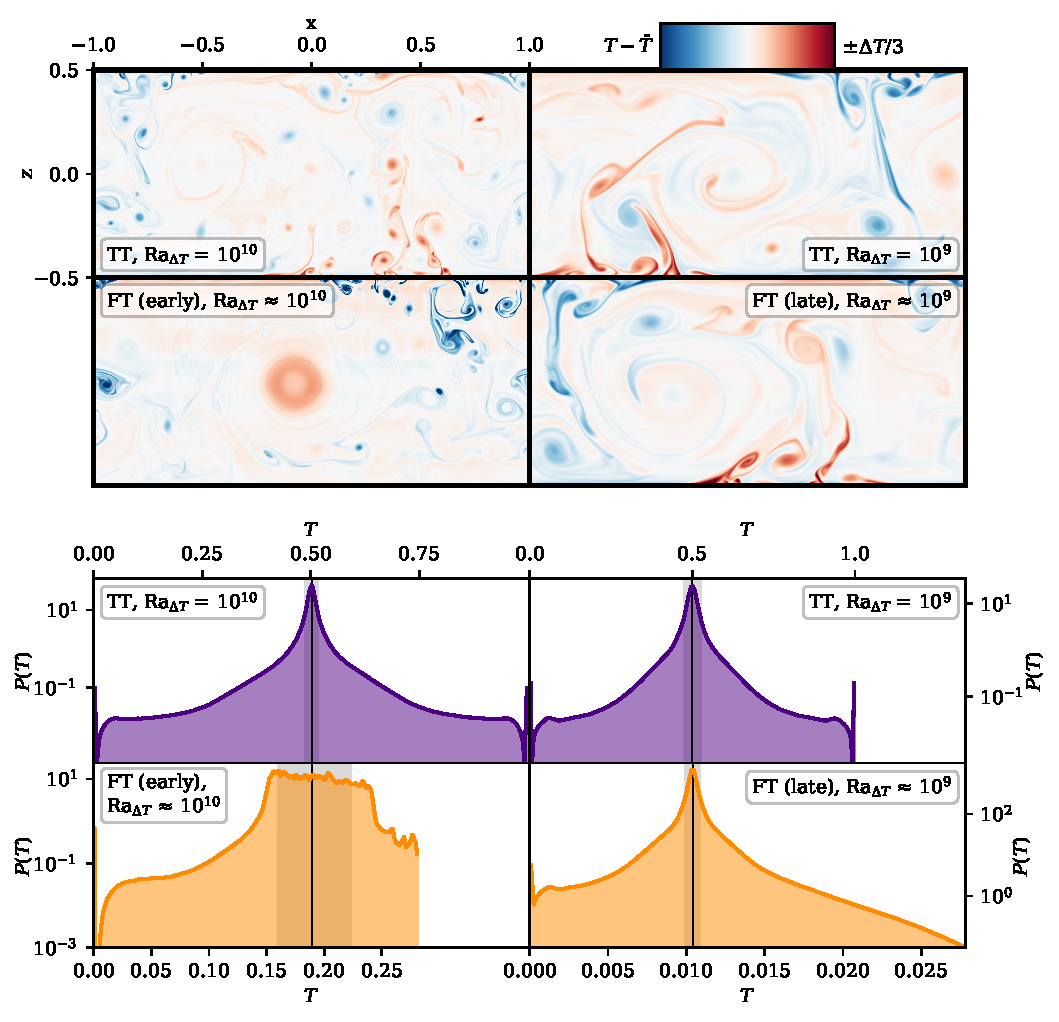
\includegraphics[width=\textwidth]{./figs/rbc_evolution_dynamics.pdf}
\caption{ 
	(Upper four panels) Snapshots of the temperature anomaly in two TT simulations (top row) and in an FT simulation (bottom row).
	The left column shows a TT case at Ra$_{\Delta T} = 10^{10}$ and the dynamics early in an FT simulation when its effective Ra$_{\Delta T} \approx 10^{10}$.
	Despite similar flow structures (a large convective cell and plumes which break apart into small turbulent eddies), the temperature anomaly of the hot plume is distinctly smaller than the cold plume in the FT case.
	The right column shows a TT case at Ra$_{\Delta T} = 10^9$, and the dynamics of the converged FT case when it has Ra$_{\Delta T} \approx 10^9$.
	The dominant asymmetries observed in the early flow have vanished, and the FT and TT case are visually indistinguishable.
	(Bottom four panels) Probability distribution functions of the temperature fields corresponding to the four simulations in the upper panels.
	(Top row) In both cases, the TT temperature field has a mean value at $T = 0.5$ and a symmetric distribution around that peak. 
	(Bottom left) At early times, A long tail reaching towards the cold (left) boundary is observed, but there is no clear mode of the PDF due to the constantly changing value of $\Delta T$ in this simulation (over time, the modal temperature moves from right to left).
	(Bottom right) At late times, the temperature PDF from the mode to the fixed-temperature (cold) boundary is indistinguishable from the TT PDF, but from the mode to the fixed-flux boundary there is a large tail characterized by low-probability, hot elements.
	\label{fig:rbc_evolution_dynamics} }
\end{figure}

In Fig.~\ref{fig:rbc_evolution_dynamics}, we compare the time-evolution of the temperature field of an FT simulation with Ra$_{\partial_z T}$ = 4.83$\,\times 10^{10}$ to two TT simulations (with Ra$_{\Delta T} = 10^{10}$ and Ra$_{\Delta T} = 10^9$, respectively).
As shown in the top four panels, in all simulations, we see a classical convective roll solution, as is anticipated for 2D RBC.
Interestingly, at early times, we find that the dynamics of the FT simulation (bottom left) is highly asymmetrical compared to a comparable TT simulation (upper left), although the size of the turbulent convective structures is similar.
In the early FT case, the temperature anomaly in the upper (cold) plume is much greater than the temperature anomaly in the warm plume.
This excess of cold material slowly fills the domain and mixes, reducing the temperature difference between the top and bottom plates from $\Delta T = 1$ to $\Delta T = \text{Nu}^{-1}$ in the final, equilibrated state.
Eventually, the supply of warm material from the bottom boundary balances the supply of cold material from the top boundary, and the temperature profile of the simulation stops drifting.
In this converged state, FT dynamics (bottom right) panel are indistinguishable from TT dynamics (top right).

When we examine these temperature fields statistically (bottom four panels), we find a similar story.
Both of the TT simulations (top row) have a mean temperature of 0.5  and some probability of hotter/colder material (mostly contained in the plumes), bounded by the fixed-temperature boundary values.
At early times (lower left), the FT simulation shows an extreme tail to its PDF that characterizes the cold plume at the upper boundary.
Furthermore, the early FT simulation has no distinct mode in its temperature PDF, but rather shows that migration of the modal temperature value from hot temperatures (on the right) toward colder temperatures.
At late times (lower right), the  FT simulation's PDF is indistinguishable from the TT PDF between the cold (left) boudnary and the modal value.
From the modal value towards warmer temperatures, we find that fixed-flux boundaries are capable of producing more extreme temperature events than fixed temperature boundaries.
This is explored further in section \ref{sec:asymmetries}.

\begin{figure}[b!]
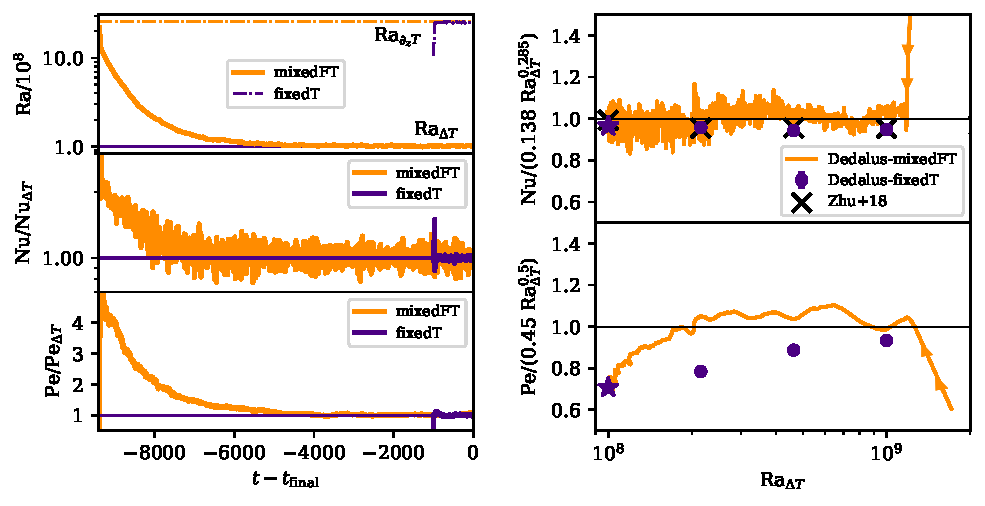
\includegraphics[width=\textwidth]{./figs/rbc_scalar_comparisons.pdf}
\caption{ 
	(left three panels) Time traces of rolling averages over 100 freefall times of an FT (orange) and a TT (purple) simulation.
	(top left panel) Ra, normalized by the input Ra$_{\Delta T}$ = $10^9$ value of the TT simulation.
	(middle and bottom left panels) The evolution of Nu and Pe is shown, and is normalized by the mean value measured over the last 500 freefall times of the TT simulation (reported in appendix \ref{app:table}).
	(right two panels) Compensated parameter space plots of Nu (upper) and Pe (lower) vs. Ra$_{\Delta T}$.
	The Nu vs Ra.~plot is compensated by $(0.138 \text{Ra}_{\Delta T}^{0.285})$, which was the best-fit reported by ref.~\cite{johnston&doering2009}.
	The Re vs Ra.~plot is compensated by a Ra$_{\Delta T}^{1/2}$ law, which is the anticipated scaling of Pe \cite{ahlers&all2009}.
	The orange trace shows the time evolution of the FT case from the left panels with the arrows showing the sense of time.
	The yellow trace shows the evolution of an FT case with Ra$_{\Delta T} = 10^8$.
	Purple circles show our measured values of Nu in TT simulations (reported in appendix \ref{app:table}); error bars show the standard deviation of the sample mean and are smaller than the marker in all cases.
	The purple circles filled in with yellow and orange are the TT comparisons for the evolved states of the two FT cases.
	Black crosses show comparison TT simulations as reported by ref.~\cite{zhu&all2018}.
\label{fig:rbc_scalar_comparisons} }
\end{figure}

In the left panels of Fig.~\ref{fig:rbc_scalar_comparisons}, we display the time evolution of scalar quantities from the FT simulation shown in Fig.~\ref{fig:rbc_evolution_dynamics} (orange lines) and compare it to the TT simulation with Ra$_{\Delta T} = 10^9$ (purples lines).
Simulation time in nondimensional freefall units is shown on the x-axis; each simulation's end time, $t_{\text{final}}$, is subtracted so that the final evolved states can be more directly compared, and so that $x = 0$ corresponds to the end of the simulation.
The lines shown are rolling averages taken over 100 freefall time units.
In the top-left panel, the evolution of Ra$_{\Delta T}$ and Ra$_{\partial_z T}$ is shown in each simulation.
In the FT simulation, Ra$_{\Delta T}$ evolves towards its final value over thousands of simulation time units; this final value corresponds to the input value of the equivalent TT case.
In comparison, Ra$_{\partial_z T}$ for the TT case nearly instantaneously reaches its final value, which corresponds to the input value for the FT simulation.
This discrepancy in evolution timescales, where TT simulations evolve quickly and FT simulations evolve slowly, is also seen in the equilibration of Nu (middle panel) and Pe (bottom panel).

The right panels of Fig.~\ref{fig:rbc_scalar_comparisons} show that the evolution of Ra$_{\Delta T}$ in FT simulations is akin to a sweep through Ra$_{\Delta T}$ parameter space.
The orange lines show the evolution of the Ra$_{\partial_z T} = 4.83 \times 10^{10}$ case shown on the left, and the yellow lines show the evolution of a Ra$_{\partial_z T} = 2.61 \times 10^{9}$.
The arrows give the sense of time in the simulations.
For comparison, we have computed TT simulations throughout this parameter space (purple circles) and we have overplotted the reported results of ref.~\cite{zhu&all2018}.
The purple circles filled with orange and yellow circles respectively show the comparison TT simulations for the evolved FT simulations.
In the upper panel, we show a compensated scaling plot for Nu vs.~Ra$_{\Delta T}$, compensated by the best fit reported in ref.~\cite{johnston&doering2009}.
The lower panel is a compensated scaling plot of Pe vs~Ra$_{\Delta T}$, compensated by the expected scaling \cite{ahlers&all2009}.
We find that the FT simulations are more turbulent (higher Pe) and carry marginally more flux (higher Nu) than comparable TT simulations as they sweep through this parameter space.
The dynamics in FT simulations evolve slowly during the rundown, and these traces demonstrate the importance of waiting until an FT simulation has reached its equilibrated state before sampling and analyzing the nonlinear convective state.
Furthermore, the heightened values of Nu and especially Pe suggest that the dynamics do not immediately ``forget'' the higher-Ra$_{\Delta T}$ state that they recently timestepped through on their way to achieving thermal relaxation.

\subsection{Evolved Structure}
\begin{figure}
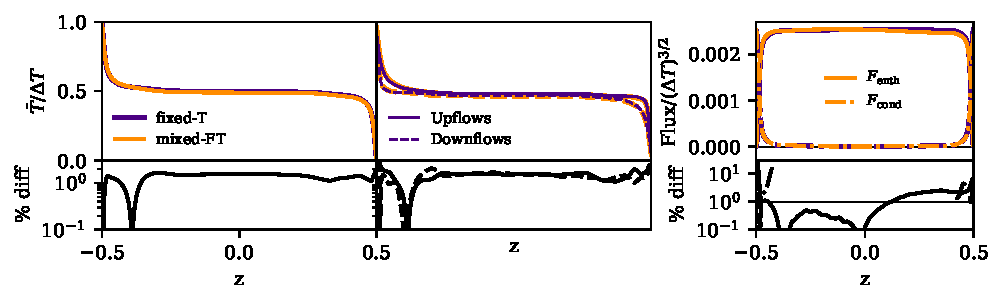
\includegraphics[width=\textwidth]{./figs/rbc_1D_profiles.pdf}
\caption{ 
	(left three panels) Shown are the time- and horizontally-averaged temperature (top), temperature in upflows and downflows (middle), and fluxes (bottom) for a TT-to-FT (orange) and TT (purple) case at Ra$_{\Delta T} = 10^{10}$.
	The boundary layer regions are separated from the bulk by thin vertical lines.
	The boundary layers are examined in more detail in the right six panels: the middle column examines the bottom boundary layers, and the right panel examines the top boundary layers.
	The insets show the \% difference between the FT and TT solutions.
	There are appreciable (a few \%) differences in two places: the enthalpy flux (likely due to a short sampling window), and in the mean temperature profiles in upflows and downflows at the bottom (fixed flux) boundary.	
\label{fig:rbc_1D_profiles} }
\end{figure}

In Fig.~\ref{fig:rbc_1D_profiles}, we compare the time- and horizontally averaged, profiles of the temperature and fluxes in the evolved FT and TT cases presented in Fig.~\ref{fig:rbc_scalar_comparisons}.
Time averages are taken over 500 nondimensional freefall time units, sampled once every 0.1 time units.
The left three panels show (top) the mean temperature profile, (middle) the mean temperature profile in the upflows (solid) and downflows (dashed), and (bottom) the convective enthalpy flux ($F_{\text{enth}} = wT$) and the conductive flux ($F_{\text{cond}} = -\Peff^{-1}\grad T$).
Most of the interesting structure of these profiles is in the boundary layers, located between the edges of the plots and the thin vertical black lines.
Zoomed in views of the bottom and top boundary layers are respectively shown in the middle and right columns.
Inset panels show the percentage difference between the FT and TT solutions.
In the case of the flux panels (bottom row), we do not show the \% difference in the conductive flux; the two cases agree to $\sim$1\% in the boundary layers, and the maximum deviation away from zero in the interior is less than 0.01. 

We find good ($\sim 1\%$) agreement between the temperature profiles throughout the full depth of the domain.
When we examine the temperature in upflows and downflows respectively, we find similarly good agreement near the upper (fixed temperature) boundary, but differences of a few percent between the FT and TT case right near the bottom boundary layer.
Specifically, we find that FT (upflows/downflows) are slightly (warmer/cooler) than their TT counterparts at the hot, bottom boundary.
These differences are interesting, and are explored further in section \ref{sec:asymmetries} and Fig.~\ref{fig:rbc_dynamics_asymmetries}, but vanish in the interior and do not likely affect the convective dynamics appreciably.
While there are very small differences between the condcutive fluxes, we do find differences between the convective fluxes of up to $\sim 3\%$ at most.
We anticipate that these differences are merely a result of a small sample of convective dynamics in the FT case and do not point to appreciably differences in the heat transport.

\subsection{TT-to-FT: Rapidly equilibrated FT simulations}


\begin{figure}
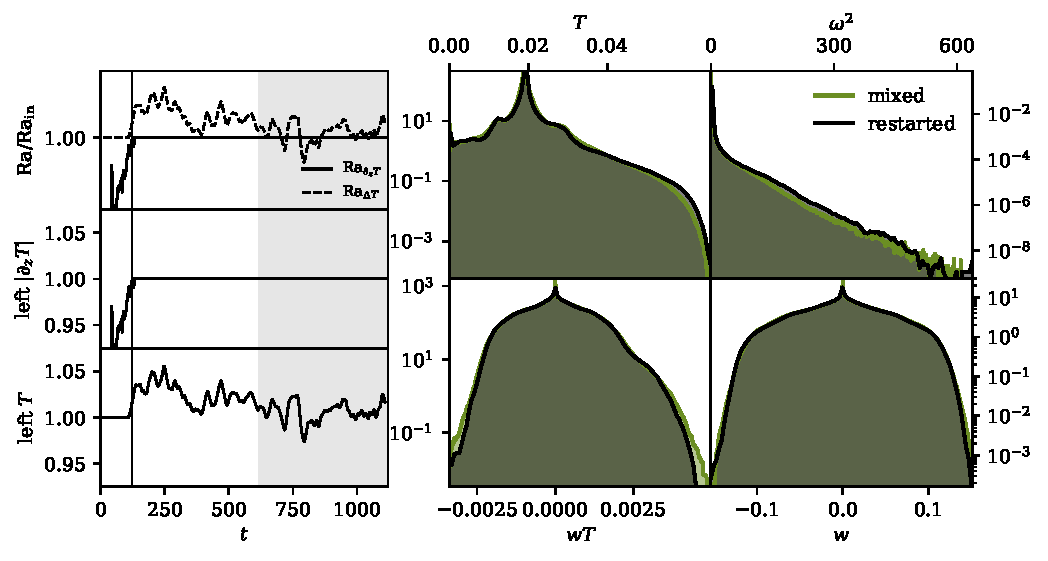
\includegraphics[width=\textwidth]{./figs/rbc_restart_description.pdf}
\caption{ 
	(left three panels) Time traces of rolling averages over 25 freefall times of a simulation with Ra$_{\Delta T} = 10^9$ which starts with TT boundary conditions and then is switched to FT boundary conditions.
	The time at which we switch from TT to FT boundaries is noted by the vertical black line.
	(top left panel) The evolution of Ra over time is shown; Ra$_{\partial_z T}/(4.83\times 10^{10})$ is shown as a dashed-dot line, while Ra$_{\Delta T}/10^9$ is shown as a solid line.
	The mean value of the bottom boundary's temperature gradient (middle panel) and temperature (bottom panel) are consistently nondimensionalized and displayed, showing the change in the enforced boundary condition.
	In the TT initial state, the temperature is held constant at a value of 1 and the temperature derivative fluctuates around a value of $\text{Nu}$.
	In the FT final state, the temperature derivative is held constant at a value of -1 and the temperature value fluctuates around a value of $\text{Nu}^{-1}$.
	(right four panels) Probability distribution functions of dynamics at all spatial points in the domain sampled once each freefall time for a total of 500 freefall times are shown (the grey shaded region in the left three panels).
	We display the temperature field (upper left), enstrophy (upper right), nonlinear convective enthalpy flux (bottom left), and vertical velocity (bottom right).
	In each plot, we compare the PDF of the FT case which thermally relaxed (in Fig.~\ref{fig:rbc_scalar_comparisons}; green PDF) to the PDF of the TT-to-FT case (grey PDF).
\label{fig:rbc_restart_description} }
\end{figure}

The equivalence of the evolved values of Ra, Nu, and Pe in Fig.~\ref{fig:rbc_scalar_comparisons} between the FT and TT simulations suggests that, in a volume-averaged sense, there is a comparable TT experiment for each FT experiment.
It should therefore be possible to take advantage of the fast evolution of TT simulations to achieve rapidly equilibrated FT simulations, which would save a great deal of computing time in solving FT simulations.
The rundown in FT simulations is very costly for two reasons: (1) the turbulent dynamics at the large initial Ra$_{\Delta T}$ require more spectral modes to resolve than the equilibrated state, and (2) thousands of freefall times must pass during relaxation.
For example, for the cases displayed in the left panels of Fig.~\ref{fig:rbc_scalar_comparisons}, with a modest Ra$_{\Delta T} = 10^9$, the full evolution of the FT simulation costs $4.75 \times 10^5$ cpu-hours, while the TT equivalent case costs $5.58 \times 10^4$ cpu-hours -- nearly an order of magnitude difference.

We now briefly describe a procedure which takes advantage of the fast evolution of TT simulations to achieve equilibrated FT simulations.
In short, the evolved flow fields in the TT simulation are properly re-nondimensionalized and used as initial conditions for an FT simulation.
Throughout this work, we will refer to simulations conducted this way as ``TT-to-FT'' simulations.
To achieve this, we perform these steps:
\begin{enumerate}
\item Run a TT simulation to its statistically stationary state ($\sim100+$ freefall time units). 
Measure $\text{Nu}$ in that state.
\item Re-nondimensionalize from $\Delta = \Delta T \rightarrow \partial_z T$, and from Ra$_{\Delta T}\rightarrow$Ra$_{\partial_z T}$, as in Eqn.~\ref{eqn:ra_relation}.
In our freefall nondimensionalization, this means setting the velocities in the FT simulation to $\bm{u}_{\text{FT}} = \bm{u}_{\text{TT}} / \sqrt{\text{Nu}}$, and setting the temperature field to $T_{\text{FT}} = T_{\text{TT}} / \text{Nu}$.
\item Restart the simulation with FT boundaries and continue timestepping.
\end{enumerate}
At the end of the Ra$_{\Delta T} = 10^9$ TT simulation shown in Fig.~\ref{fig:rbc_scalar_comparisons}, we change the boundary conditions to FT at Ra$_{\partial_z T} = 4.83\times 10^{10}$ and restart the simulation using the above procedure.
In the left panels of Fig.~\ref{fig:rbc_restart_description}, we show the temporal behavior of Ra (top panel), the flux at the bottom boundary (middle panel), and the temperature difference between the top and bottom boundaries (bottom panel).
The change from TT to FT boundaries is shown by the thin vertical line.
Unlike in the FT case displayed in Fig.~\ref{fig:rbc_scalar_comparisons}, there is no long thermal rundown in the FT state, due to the rapid relaxation achieved during the TT portion of the simulation.

In the right four panels of Fig.~\ref{fig:rbc_restart_description}, we compare probability distribution functions (PDFs) of flow fields in this TT-to-FT simulation and the comparable FT simulation shown in Fig.~\ref{fig:rbc_restart_description}.
To create these PDFs, we sample the full simulation flow field once every simulation freefall time unit over the final 500 time units of each simulation (e.g., the grey shaded region in the left panels of Fig.~\ref{fig:rbc_restart_description}).
We interpolate the (unevenly spaced) vertical Chebyshev gridpoints onto an evenly spaced grid before histogramming the flow values.
Shown are PDFs of the temperature field (upper left), enstrophy (upper right), convective flux (lower left), and vertical velocity (lower right).
In Table~\ref{table:pdf_values}, we display the first four moments of each of these distributions,
\begin{equation}
\begin{split}
&\mu(A) \equiv \sum_{i} A_i\,P(A_i)\,\Delta A,\qquad\qquad\qquad\qquad\qquad\qquad\,\,
\sigma(A) \equiv \sqrt{\sum_{i}[A_i-\mu(A)]^2 P(A_i) \Delta A},\\
&\text{Skewness}(A) \equiv \frac{1}{\sigma(A)^3}\sum_i [A_i-\mu(A)]^3 P(A_i) \Delta A,\qquad
\text{Kurtosis}(A) \equiv \frac{1}{\sigma(A)^4}\sum_i [A_i-\mu(A)]^4 P(A_i) \Delta A,
\end{split}
\label{eqn:pdf_moments}
\end{equation}
where $A$ is a flow quantity, $P(A)$ is the PDF of $A$, $\mu$ is the mean, $\sigma$ is the standard deviation, $\Delta A$ is the spacing between the discrete PDF bins, and $i$ is the index of the bin.
The PDFs are qualitatively similar, and there is generally good agreement between the moments of the PDFs.
The FT simulation here is not perfectly converged to many decimal places; the few \% difference between the modal values of the temperature PDFs is due to this lack of perfect convergence, and given infinite time the peak of the green FT PDF would shift left.
The remaining discrepancies between the PDFs are small and seem to primarily be due to the randomness of the flows in the time windows over which we sampled the simulations.

\begin{table}[t!]
\caption{ 
	The first four moments, as defined in Eqn.~\ref{eqn:pdf_moments}, of each of the PDFs shown in Fig.~\ref{fig:rbc_restart_description} are displayed below.
}
\setlength{\tabcolsep}{12pt}
\label{table:pdf_values}
\begin{center}
\begin{tabularx}{\textwidth}{c c c c c c}
\hline																	
Quantity &	Case	&	$\mu$	&	$\sigma$	&	Skewness	&	Kurtosis \\
%\hline \hline \multicolumn{6}{c}{\vspace{-0.2cm}}\\
%\multicolumn{6}{c}{\vspace{0.1cm}2D Runs} \\
\hline
$T$				&	FT			&		$1.11 \times 10^{-2}$	&	$1.53 \times 10^{-3}$	&	0.179		&	26.5 \\
				&	TT-to-FT	&		$1.05 \times 10^{-2}$	&	$1.53 \times 10^{-3}$	&	0.729		&	26.8 \\
\hline
$\omega^2$		&	FT			&		$20.2$					&	$9.66$					&	71.4		&	$9.65\times 10^3$ \\
				&	TT-to-FT	&		$28.6$					&	$10.0$					&	96.8		&	$1.97 \times 10^4$ \\
\hline
$wT$			&	FT			&		$4.51 \times 10^{-6}$	&	$5.43 \times 10^{-4}$	&	0.0437	&	$2.99$ \\
				&	TT-to-FT	&		$4.40 \times 10^{-6}$	&	$5.08 \times 10^{-4}$	&	0.0114	&	$3.07$ \\
\hline
$w$				&	FT			&		$1.56 \times 10^{-5}$	&	$4.86 \times 10^{-2}$	&	0.0133	&	$2.92$ \\
				&	TT-to-FT	&		$-1.74 \times 10^{-5}$	&	$4.82 \times 10^{-2}$	&	-0.0174	&	$3.02$ \\
\hline																	
\end{tabularx}
\end{center}
\end{table}

We note briefly that this mechanism that we describe here is not the only mechanism for accelerating the thermal relaxation of an FT simulation.
We discuss other mechanisms, and explore one in detail, in our previous work \cite{anders&all2018}.
We note however that the TT-to-FT setup described here is likely the least complicated mechanism for achieving rapid relaxation in a simplified \RB convection setup that we are aware of.
The successful degree with which this mechanism reproduces the evolved dynamics suggests that thermal relaxation occurs in two parts:
\begin{enumerate}
\item Changes to the simulation energy reservoir, and
\item Restratification of the experiment.
\end{enumerate}
The rapid evolution of TT runs, whose energy reservoir does not change between the initial and final state, suggests that experimental restratification occurs rapidly in RBC. 
The long rundown of FT experiments on display in Fig.~\ref{fig:rbc_scalar_comparisons} is entirely due to the energy reservoir (the mean temperature) drifting over time.
Put differently, the classic \RB setup for $T_0(z)$ is a bad choice of initial conditions for FT boundaries, and TT-to-FT simulations use TT dynamics to choose a more ideal set of initial conditions.


\subsubsection{Changing Timescales}
\label{sec:timescales}
One surprising result of our FT simulations is that the nondimensional dynamical freefall timescale is a poor description of the \emph{evolved} freefall timescale.
As noted above in our TT-to-FT procedure, the velocities in an FT simulation are smaller than the velocities in a TT simulation by a factor of $\sqrt{\text{Nu}}$.
This implies that every nondimensional freefall time in a TT simulation samples a factor of $\sqrt{\text{Nu}}$ more dynamics than a nondimensional freefall time in an FT simulation.
This is on display in Fig~\ref{fig:rbc_restart_description}, where the flow variations occur at a higher frequency in the TT portion of the simulation than in the FT portion.
However, we note briefly that in FT simulations, Ra$_{\partial_z T}$ is the input Ra, and it is larger than Ra$_{\Delta T}$ by a factor of $\text{Nu}$.
Thus, the \emph{thermal diffusion timescale}, which scales like $\sqrt{\text{Ra}_{\text{input}}}$, is also larger in FT simulations by a factor of $\sqrt{\text{Nu}}$.
This means that one convective overturn timescale occurs over the same fraction of a nondimensional \emph{diffusion} timescale regardless of boundary conditions or temperature nondimensionalization.
These results suggest that comparisons of systems which are nondimensionalized on the flux and the temperature may be more straightforward in a thermal diffusion nondimensionalization \cite{goluskin2015} than the freefall nondimensionalization we have used throughout this work.

\subsection{Asymmetries induced by mixed boundaries}
\label{sec:asymmetries}

\begin{figure}
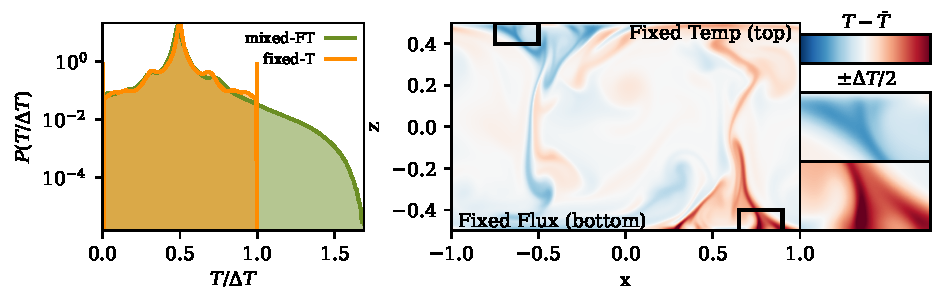
\includegraphics[width=\textwidth]{./figs/rbc_dynamics_asymmetries.pdf}
\caption{ 
	(left panel) PDFs of temperature measurements of a TT-to-FT (orange) and TT (purple) case with Ra$_{\Delta T} = 10^{10}$ are displayed.
	The right tail of the distribution (near the hot fixed-flux boundary for the FT case) shows that fixed flux boundaries achieve more extreme temperature events than fixed temperature boundaries.
	(middle panel) A snapshot of the temperature anomaly in the FT simulation.
	The black outline boxes around the roots of the plumes are zoomed in in the right two panels.
	Near the top (fixed temperature) boundary, the temperature anomaly at the root of the plume vanishes near the boundary, but this does not happen near the bottom (fixed flux) boundary, allowing for more extreme instantaneous values.
\label{fig:rbc_dynamics_asymmetries} }
\end{figure}

We now study in more detail the asymmetries introduced into a solution by FT boundaries.
We run a TT and TT-to-FT simulation at Ra$_{\Delta T} = 10^{10}$ and Ra$_{\partial_z T} = 9.51 \times 10^{11}$, respectively.
In Fig.~\ref{fig:rbc_dynamics_asymmetries}, we examine the dynamical nature of the asymmetries which FT boundaries introduce into the simulation near the fixed-flux boundary.
In the left panel, we plot PDFs of the temperature fields in comparable TT and FT simulations.
These PDFs agree remarkably well near the mean and for cold temperatures (near the fixed temperature boundary), but diverge in the tail of the PDF for hot temperatures where $T/\Delta T \gtrsim 0.8$, where the boundary conditions differ.
Interestingly, there are no temperature fluctuations which exceed the specified boundary values in the convective domain for TT simulations.
However, the FT PDF has a much longer tail and the FT solution achieves fluid parcels which are hotter than the average bottom boundary value by more than 50\%.
In order to understand how this is possible, we examine a snapshot of the full temperature field.
In the middle panel, we plot the temperature anomaly, or the temperature field with the mean vertical profile subtracted from it.
We have outlined a portion of a cold plume near the upper (fixed-temperature) boundary and a portion of a hot plume near the lower (fixed-flux) boundary, and these regions are magnified in the rightmost panels.
The TT upper boundary suppresses temperature anomaly at the upper boundary and regulates the temperature minima which can be achieved.
The fixed-flux lower boundary does no such suppression and allows for extreme temperature values to be achieved in the plume-launching area, thus allowing for the asymmetry in the tails of the temperature PDF.

We note briefly that these asymmetries do not seem to affect mean or volume-averaged quantities in these simulations appreciably (see the agreement between FT and TT in Figs.~\ref{fig:rbc_scalar_comparisons}\&\ref{fig:rbc_1D_profiles}).
However, the fact that fixed-flux boundaries produce a wider temperature distribution with more extreme values may be important in some astrophysical studies.
We explore this further in the discussion in section \ref{sec:discussion}.





\section{Rotating \RB Convection}
\label{sec:rotating_results}
\begin{figure}
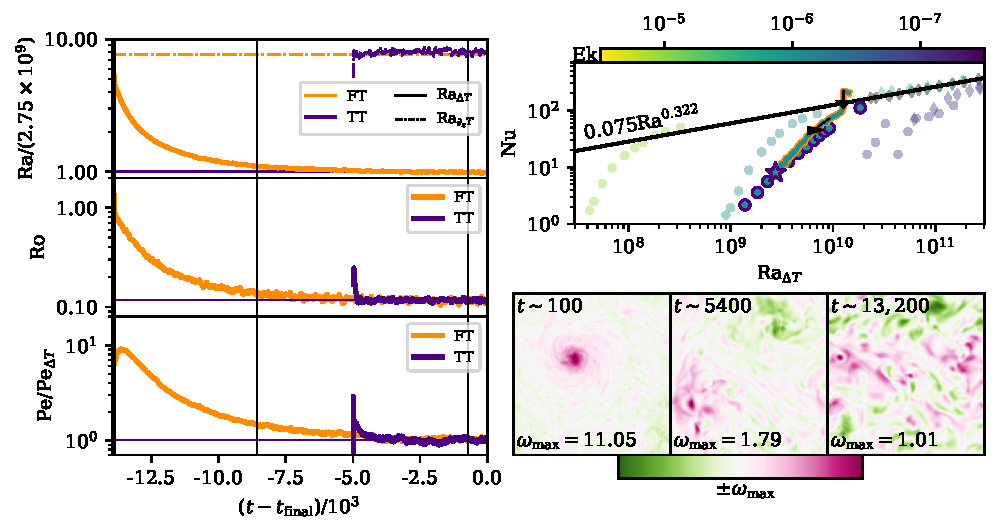
\includegraphics[width=\textwidth]{./figs/rotating_panels.pdf}
\caption{ 
	(left three panels) Time traces of rolling averages over 50 freefall times of a rotating FT simulation (green) and a TT (orange) simulation.
	(top left panel) Ra, normalized by the input Ra$_{\Delta T}$ = 2.75$\,\times 10^9$ of the TT simulation.
	(middle left panel) Ro evolution of both simulation; the bulk flow of the FT simulation transitions from a marginally rotationally constrained state to a heavily constrained state, while the TT simulation is in this latter state through its full evolution.
	(bottom left panel) Pe evolution of the simulations is shown, normalized by the mean value measured over the last 500 freefall times of the TT simulation.
	(right upper panel) Parameter space plots of Nu vs.~Ra$_{\Delta T}$.
	Circlular and diamond data points are respectively simulations and experimental data points from \cite{cheng&all2015}.
	The color of the data points signifies the Ekman number of the points, and black points are nonrotating.
	Data from our FT experiment are shown as a thick orange line with a cyan interior, and the corresponding TT experiment's average is shown as a purple star with a cyan interior.
	Some comparison TT simulations through this parameter space are shown as purple circles with a cyan interior.
	(Bottom right panels) Snapshots of the vertically integrated z-component of the vorticity from the FT simulation.
	At early times (left panel), a powerful large scale vortex with positive vorticity develops.
	This vortex slowly decays and becomes a vortex pair (middle panel), as seen in ref.~\cite{stellmach&all2014}.
	In the converged state, we see oscillatory behavior between this vortex pair behavior and jets (right panel).
	The TT case exhibits the oscillatory behavior between vortex pairs and jets throughout its whole evolution.
	The three vertical black lines in the left panels signify the times at which this snapshots are taken.
\label{fig:rotating_panels} }
\end{figure}



We now extend our study to a more complicated experiment: 3D rotating RBC with an Ekman number of $10^{-6}$.
We study a TT case at Ra$_{\Delta T} = 2.75\times 10^9$, and an FT case at $\text{Ra}_{\partial_z T} = 2.1 \times 10^{10}$ (the supercriticality of the TT case is $\sim 3$).
These simulations employ stress free boundary conditions which allow for the generation of mean flows such as large scale vortices (LSV) \cite{couston&all2019}.

In the left three panels of Fig.~\ref{fig:rotating_panels}, we compare the time evolution of the FT and TT cases.
The top left panel shows the evolution of Ra$_{\partial_z T}$ and Ra$_{\Delta T}$.
Even in the presence of strong rotation, the TT case's fluxes immediately equilibrate, but the FT case takes thousands of freefall times to achieve thermal relaxation.
In the middle panel, we show the evolution of Ro; the evolved flows in both simulations exhibit rotationally constrained dynamics with Ro $\,\approx 0.1$, the flows in the FT simulation initially experience weak rotational influence (Ro $\,\approx 1$).
In the bottom panel, we display the evolution of Pe over time.
Strangely, the peak value of Pe occurs a few hundred freefall times after the convective transient.
After achieving this peak value, Pe monotonically decreases toward its equilibrium state.

In the upper right panel of Fig.~\ref{fig:rotating_panels}, we plot a parameter space cut of Nu vs.~Ra for rotating simulations.
We have evolved select TT cases, and their values are plotted as cyan circles with purple outlines (where here, the cyan shows the value of Ek for the simulations, per the colorbar).
The evolution of the FT case in the left panels is shown as a thick orange line with a cyan interior, and the corresponding TT case is shown as a cyan star with a purple outline.
We have additionally included some literature data from numerical simulations (circles) and experiments (diamonds) as reported in the appendix tables of ref.~\cite{cheng&all2015}.
These experiments were conducted in a cylindrical geometry at a different Pr, and are not meant to be one-to-one-comparable, but are meant to guide the eye to the nature of the parameter space of rotating convection.
The solid black line is the best-fit line for rotationally unconstrained simulations with Ra $\geq 10^{10}$ from ref.~\cite{cheng&all2015}.
As expected, the scaling of Nu vs.~Ra is steep in the rotationally constrained regime \cite{julien&all2012, plumley&julien2019}, which these simulations trace through.
As in Fig.~\ref{fig:rbc_scalar_comparisons}, the FT values of Nu are once again somewhat elevated above the comparable TT simulations.

In the bottom right three panels of Fig.~\ref{fig:rotating_panels}, we plot the vertically integrated vertical vorticity in the simulation at three different times.
In the left panel, a dominant LSV which is aligned with the global rotation dominates the simulation at early times.
Over thousands of freefall times, this LSV evolves into a long-lived vortex pair, displayed in the middle panel.
Finally, in the evolved state, this vortex pair solution begins to oscillate with domain-wide jets, such as those displayed in the right panel.
We find that the the TT solution shows this oscillatory behavior between vortex pairs and jets immediately and throughout the full 5000 frefall timescales of evolution that we simulated.

We suspect that the evolution of the dominant flow structures over time explains the strange behavior of Pe in the bottom left panel.
At early times, the initially large value of Ra$_{\Delta T}$ in the FT case drives the displayed dominant LSV.
This powerful driving injects energy into the LSV, causing Pe to grow.
As Ra$_{\Delta T}$ and convective driving decrease over time, the LSV saturates and then starts to wind down, leading to the ``bump'' in the Pe trace.

We once again find it important to briefly note the difference in computational cost between the FT and TT simulations conducted here.
The TT simulation shown in the left panels of Fig.~\ref{fig:rotating_panels} only cost $2.6 \times 10^4$ cpu-hours.
By comparison, the cost of the FT simulation shown in the same panels was \emph{two orders of magnitude larger}---$2.3 \times 10^6$ cpu-hours.
The TT simulation's coefficient resolution was $128^3$.
The FT simulation's initial resolution required to resolve the convective transient was $512\times384^2$ coefficients.
We reduced the resolution to $256\times384^2$ after 100 freefall times, and then later to $128\times384^2$ after $\sim3.3 \times 10^3$ freefall times.
At each of these times, we found that lowering the \emph{horizontal} coefficient resolution of the simulation did not reproduce the simulation solution with fidelity.
This suggests that small scale turbulent velocity structures---which are injected by the vigorous transient and perhaps associated with the LSV---are long lived throughout the thermal evolution of the simulation.


%%%%%%%%%%%%
%%%%%%%%%%%
% CONCLUSION
%%%%%%%%%%%
%%%%%%%%%%%%

\section{Conclusions \& Discussion}
\label{sec:discussion}
In short, we find that FT experiments experience a long thermal relaxation which is not experienced by TT simulations and, to first order, do not introduce important asymmetries into the solution.

In this paper, we have studied the time evolution of \RB convection (RBC) under two different formulations of the thermal boundary conditions: ``FT'' boundaries, where the flux is fixed at the bottom and temperature is fixed at the top, and ``TT'' boundaries, where temperature is fixed at the top and bottom.
Through studying this relaxation and the relaxed states of both simulations, we come to the following conclusions:
\begin{enumerate}
\item Thermal relaxation in RBC has two components: (a) changes in the energy reservoir and (b) changes in the stratification.
We find that the long relaxation of FT simulations is due to changes in the energy reservoir; this reservoir is roughly constant in TT simulations due to the lack of evolution of the average domain temperature.
The rapid evolution of our TT simulations suggests that RBC restratifies itself nearly instantaneously.
\item Dynamical measurements taken during the thermal relaxation of an FT simulation may be misleading.
Dynamics during the relaxation are in a more turbulent state than in the evolved state, and can even feel different flow balances in the equation of motion (as quantified by e.g., the Rossby number).
\item The thermal relaxation process of an FT simulation performs a sweep through Ra$_{\Delta T}$ parameter space.
We find that convective heat transport (the Nusselt number) and turbulent velocities (the P\'{e}clet number) are elevated above classical scaling laws along these parameter space sweeps.
\item Great computational expense achieving thermal relaxation in an FT simulation can be avoided by using the evolved state of a TT simulation as a ``better'' set of initial conditions for an FT simulation.
\item Despite minor asymmetries near the fixed-flux boundary, we find no meaningful difference between the mean state of FT and TT simulations.
\end{enumerate}
We now describe some lessons that should be applied from this work to astrophysical convection, and comment on some open areas of research.

Throughout this work, we have made the assumption that convection is only ``interesting'' in its final, fully equilibrated state.
In nature, convection is not always in an equilibrium state.
For example, in the late stages of the lifetimes of stars, some core burning regions have sufficiently short lifetimes that they likely do not come into thermal relaxation \citep{clarkson&all2018, andrassy&all2020}.
The use of FT boundaries or initial conditions that we have here considered to be ``bad'' choices may help in understanding these transient lifetime stages.
However, for most convective studies where the lifetime of the natural convective system is much larger than its Kelvin-Helmholtz timescale, it is essential to study relaxed convection, and our results point towards the importance of either choosing good initial conditions (TT or TT-to-FT simulations) or running simulations to thermal relaxation.

One question which our study of RBC is not able to address is: how long does it take for a complex convective system to restratify?
Our fully convective domains restratified instantaneously, but it is likely that mixed convective-and-stably-stratified domains \citep{brummell&all2002, kapyla&all2019, pratt&all2017, korre&all2019} should have regions that are not turbulently mixed by convection which could also have long relaxation timescales.
It would be extremely helpful for future studies to examine relaxational timescales in systems where the energy reservoir is fixed, but where convection does not effectively mix the whole domain.
Fortunately, clever techniques (e.g., as we explored in ref.~\cite{anders&all2018}) can likely be used to rapidly restratify atmospheres in such simulations.

RBC is fundamentally symmetrical, but many natural convective processes occur in density-stratified domains in which the symmetries of the problem are fundamentally broken.
In the present study, we observed that flux boundaries produce more extreme thermodynamic events than temperature boundaries.
In studies of overshooting convection, it is possible that plumes produced by a flux boundary layer could launch further into a stable layer than plumes produced by a temperature boundary.
Some authors have aimed to quantify the nature of overshooting plumes from a convective region into a stable region \cite{pratt&all2017, korre&all2019}, and it is unclear if different choices of boundary conditions could change the observed distribution of overshooting plumes observed there.

Some of the most complex astrophysical convection experiments aim to understand self-consistently evolving magnetic dynamos in rotating, spherical, magnetohydrodynamical domains \cite{brown&all2010, yadav&all2016, strugarek&all2017, strugarek&all2018}.
These dynamo simulations involve large numbers of timesteps through many freefall timescales in order to study the generation and evolution of magnetic fields and mean flows.
We found in our FT rotating simulation that the unrelaxed state generated a mean flow (a LSV, Fig.~\ref{fig:rotating_panels}) that was much more intense and large-scale than the eventual flows that developed in the relaxed state.
If we had terminated our FT rotating simulation too early, we would not have seen the eventual destruction of this LSV or the later oscillatory behavior between jets and vortex pairs.
Many dynamo simulations are performed in highly turbulent regimes at the cutting-edge of what is achievable using modern computational resources.
As a result, timestepping through thousands of freefall timescales is not possible in these simulations.
It is therefore crucial that dynamo simulations be set up in such a manner as to avoid large changes to the system's energy reservoir such as those that we observed and studied here.
Some authors who study astrophysical convection \citep{featherstone&hindman2016a, strugarek&all2018, bordwell&all2018, matilsky&all2019} employ FF boundary conditions, and our results here suggest that such a choice may be ideal in those complex simulations.

In conclusion, we note that our results here should provide astrophysical convection simulations with reason for optimism.
Through a careful understanding of the setup of our numerical experiments, some problems that we encounter (e.g., long thermal rundown in FT simulations) can be completely avoided through a careful understanding of the system being solved.

\begin{acknowledgments}
We'd like to thank Daniel Lecoanet, who first pointed out to us the importance of examining Ra$_{\Delta T}$ in FT simulations. 
EHA acknowledges that this work was supported by NASA Headquarters under the NASA Earth and Space Science Fellowship Program -- Grant 80NSSC18K1199.
This work was additionally supported by NASA LWS grant NNX16AC92G and by the National Science Foundation under grant No.~1616538. 
Computations were conducted with support by the NASA High End Computing (HEC) Program through the NASA  Advanced Supercomputing (NAS) Division at Ames Research Center on Pleiades with allocation GID s1647.
\end{acknowledgments}


\bibliography{biblio.bib}

\appendix
\section{Table of Simulations}
\label{app:table}


\begin{table}[ht]
\caption{
	Input and output values from the simulations in this work are shown; all simulations have a Prandtl number of 1.
	The ``Nu comp'' values are comparison Nusselt number values reported in \cite{zhu&all2018}.
	Values of Nu and Re are the sample mean; the standard deviation of the sample mean is shown for Nu measurements, and is smaller than the number of significant figures reported for Re measurements.
	Resolutions marked by a $*$ show the initial, highest resolution utilized in the simulation.
	The 2D FT Ra = $4.83 \times 10^{10}$ simulation's resolution was changed to $1024\times2048$ about 500 freefall time units after transient.
	The rotating FT case's resolution was reduced to $256\times384^2$ about one hundred freefall time units after transient, and was further reduced to $128\times384^2$ about $3.3\times 10^3$ freefall times after transient.
	``TT-to-FT'' simulations are FT simulations which use an evolved TT simulation as initial conditions, and their cpu-hour cost does not include the cost of the TT transient.
}
\setlength{\tabcolsep}{8pt}
\label{table:speed}
\begin{center}
\begin{tabularx}{\textwidth}{c c c c c c c c}
\hline																	
BCs	&	Ra	&	nz$\times$nx$\times$ny	&	cpu-hours &	Nu	&	Nu comp	&	Pe  & Ro \\
\hline \hline \multicolumn{6}{c}{\vspace{-0.2cm}}\\
\multicolumn{7}{c}{\vspace{0.1cm}2D Runs ($\Gamma = 2$, no-slip)} \\
\hline
TT			&	$1.00 \times 10^8$		&	512x1024	&	$5.57 \times 10^3$	&	$25.4 \pm 0.1$	&	26.1	&	$3.18 \times 10^3$ & --- \\
FT			&	$2.61 \times 10^9$		&	1024x2048	&	$1.21 \times 10^5$	&	$25.3 \pm 0.2$	&	26.1	&	$3.31 \times 10^3$ & --- \\
TT-to-FT	&	$2.61 \times 10^9$		&	512x1024	&	$1.88 \times 10^3$	&	$26.1 \pm 0.1$	&	26.1	&	$3.22 \times 10^3$ & --- \\
TT			&	$2.15 \times 10^8$		&	512x1024	&	$5.73 \times 10^3$	&	$31.3 \pm 0.2$	&	31.2	&	$5.17 \times 10^3$ & --- \\
TT			&	$4.64 \times 10^8$		&	1024x2048	&	$4.66 \times 10^4$	&	$38.4 \pm 0.3$	&	38.9	&	$8.60 \times 10^3$ & --- \\
TT			&	$1.00 \times 10^9$		&	1024x2048	&	$5.58 \times 10^4$	&	$48.0 \pm 0.4$	&	48.3	&	$1.33 \times 10^4$ & --- \\
FT			&	$4.83 \times 10^{10}$	&	2048x4096*	&	$4.75 \times 10^5$	&	$48.7 \pm 0.4$	&	48.3	&	$1.41 \times 10^4$ & --- \\
TT-to-FT	&	$4.83 \times 10^{10}$	&	1024x2048	&	$1.11 \times 10^4$	&	$48.7 \pm 0.3$	&	48.3	&	$1.36 \times 10^4$ & --- \\
TT			&	$2.15 \times 10^9$		&	1024x2048	&	$6.38 \times 10^4$	&	$60.4 \pm 0.5$	&	61.1	&	$1.99 \times 10^4$ & --- \\
TT			&	$4.64 \times 10^9$		&	1536x3072	&	$3.29 \times 10^5$	&	$75.2 \pm 0.6$	&	76.3	&	$2.94 \times 10^4$ & --- \\
TT			&	$1.00 \times 10^{10}$	&	2048x4096	&	$7.79 \times 10^5$	&	$95.3 \pm 0.7$	&	95.1	&	$4.30 \times 10^4$ & --- \\
TT-to-FT	&	$9.51 \times 10^{11}$	&	2048x4096	&	$7.91 \times 10^4$	& 	$93.2 \pm 0.8$ 	&	95.1	&	$4.11 \times 10^4$ & --- \\
\hline																	
\multicolumn{7}{c}{\vspace{0.1cm}3D Rotating Runs (Ek = $10^{-6}$, $\Gamma = 0.481$, stress-free)} \\
\hline																	
TT	&	$1.38 \times 10^9$		&	128$\times$64$^2$	&	$2.98 \times 10^3$	&	$2.17$			&	---		&	$2.84 \times 10^2$  & $(3.38 \pm 0.17) \times 10^{-2}$ \\
TT	&	$1.83 \times 10^9$		&	128$\times$64$^2$	&	$3.54 \times 10^3$	&	$3.56$			&	---		&	$5.28 \times 10^2$  & $(5.67 \pm 0.33) \times 10^{-2}$ \\
TT	&	$2.29 \times 10^9$		&	128$^3$				&	$1.08 \times 10^4$	&	$5.61$			&	---		&	$8.91 \times 10^2$  & $(8.56 \pm 0.44) \times 10^{-2}$ \\
TT	&	$2.75 \times 10^9$		&	128$^3$				&	$2.6 \times 10^4$	&	$8.04 \pm 0.01$	&	---		&	$1.71 \times 10^3$  & $(1.17 \pm 0.06) \times 10^{-1}$ \\
FT	&	$2.1 \times 10^{10}$	&	512$\times$384$^2$*	&	$2.3 \times 10^6$	&	$7.86 \pm 0.01$	&	---		&	$1.76 \times 10^3$  & $(1.14 \pm 0.06) \times 10^{-1}$ \\
TT	&	$3.67 \times 10^9$		&	128$^3$				&	$1.55 \times 10^4$	&	$12.5$			&	---		&	$3.39 \times 10^3$  & $(1.74 \pm 0.08) \times 10^{-1}$ \\
TT	&	$4.58 \times 10^9$		&	128$^3$				&	$1.69 \times 10^4$	&	$17.6$			&	---		&	$4.77 \times 10^3$  & $(2.35 \pm 0.08) \times 10^{-1}$ \\
TT	&	$5.50 \times 10^9$		&	192$^3$				&	---					&	$22.6$			&	---		&	$6.36 \times 10^3$  & $(2.95 \pm 0.11) \times 10^{-1}$ \\
TT	&	$6.42 \times 10^9$		&	192$^3$				&	---					&	$29.3$			&	---		&	$7.84 \times 10^3$  & $(3.64 \pm 0.15) \times 10^{-1}$ \\
TT	&	$7.33 \times 10^9$		&	256$^3$				&	---					&	$36.1$			&	---		&	$9.11 \times 10^3$  & $(4.31 \pm 0.16) \times 10^{-1}$ \\
TT	&	$8.25 \times 10^9$		&	256$^3$				&	---					&	$43.0$			&	---		&	$*1.03 \times 10^4$ & $(4.98 \pm 0.21) \times 10^{-1}$ \\
TT	&	$9.17 \times 10^9$		&	256$^3$				&	---					&	$48.9$			&	---		&	$*1.15 \times 10^4$ & $(5.60 \pm 0.23) \times 10^{-1}$ \\
TT	&	$1.834 \times 10^{10}$	&	256$^3$				&	---					&	---				&	---		&	--- & --- \\
\hline																	
\end{tabularx}
\end{center}
\end{table}



\end{document}
